\documentclass{standalone}
\usepackage{tikz}
\usepackage{pgfplots}
\pgfplotsset{compat=1.18}
\begin{document}

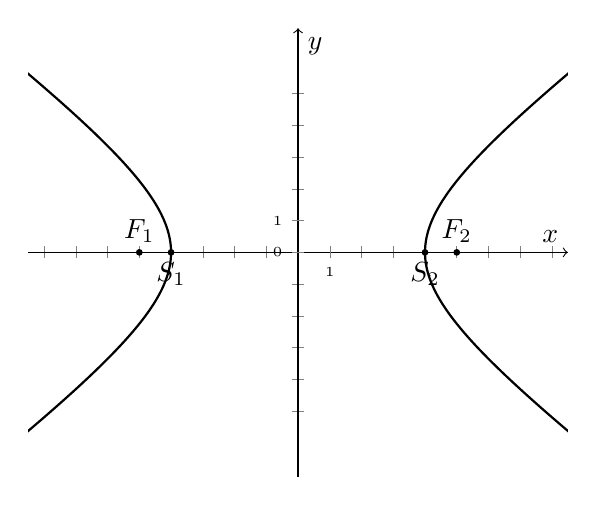
\begin{tikzpicture}[scale=1]
\begin{axis}[
    xmin=-8.5, xmax=8.5,
    ymin=-5, ymax=5,
    axis lines=middle,
    axis line style={->},
    ticklabel style={font=\tiny},
    axis equal,
    xtick={-8,-7,-6,-5,-4,-3,-2,-1,0,1,2,3,4,5,6,7,8},
    ytick={-5,-4,-3,-2,-1,0,1,2,3,4,5},
    extra x ticks={1},
    extra y ticks={0,1},
    xticklabels=\empty,
    yticklabels=\empty,
    xlabel={$x$},
    ylabel={$y$}
]

% Parameters
\def\a{4}
\def\b{3}
\pgfmathsetmacro{\c}{sqrt(\a*\a + \b*\b)} % c = 5

% Right branch
\addplot [domain=0:1.5, samples=100, thick] 
    ({\a*cosh(x)}, {\b*sinh(x)});
% Left branch
\addplot [domain=0:1.5, samples=100, thick] 
    ({-\a*cosh(x)}, {\b*sinh(x)});

% Bottom halves
\addplot [domain=0:1.5, samples=100, thick] 
    ({\a*cosh(x)}, {-\b*sinh(x)});
\addplot [domain=0:1.5, samples=100, thick] 
    ({-\a*cosh(x)}, {-\b*sinh(x)});

% Foci
\filldraw (axis cs:\c,0) circle (1pt);
\node[above] at (axis cs:\c,0) {$F_2$};
\filldraw (axis cs:-\c,0) circle (1pt);
\node[above] at (axis cs:-\c,0) {$F_1$};

% Vertices
\filldraw (axis cs:\a,0) circle (1pt);
\node[below] at (axis cs:\a,0) {$S_2$};
\filldraw (axis cs:-\a,0) circle (1pt);
\node[below] at (axis cs:-\a,0) {$S_1$};

% Conjugate rectangle points
%\filldraw (axis cs:0,\b) circle (1pt);
%\node[above left] at (axis cs:0,\b) {$S_3$};
%\filldraw (axis cs:0,-\b) circle (1pt);
%\node[below left] at (axis cs:0,-\b) {$S_4$};

\end{axis}
\end{tikzpicture}

\end{document}